%!TEX root = ..\MainFile.tex
\section{Модели ``с вязкостью''} % (fold)
\label{sec:ClassicalModelsWIthViscosity}
	\subsection{Феноменологические уравнения} % (fold)
	\label{sub:TonerAndTu}
		Основываясь на соображениях симметрии и используя методы теории ренормализационных групп, Tu~\cite{tu2000} выписал обобщенные уравнения движения для систем, состоящих из частиц, взаимодействующих по правилу Viksec'a, рассмотреному в разделе~\ref{sec:CompModelsBasics}. 

		Им были отмечены следующие общие характеристики, которыми обладают все компьютерные модели групповой динамики, а именно:
		\begin{enumerate}
			\item большое число точечных частиц (``боидов'') перемещается со временем в пространстве, стремясь ``следовать'' (т.е. двигаться в одном направлении) за своими соседями
			\item взаимодействие короткодействующее: каждый ``боид'' реагирует на окружение внутри определенного малого радиуса $R$
			\item ``следование'' не совершенно - каждый ``боид'' постоянно совершает ошибки, которые моделируются белым шумом
			\item модель обладает полной вращательной симметрией - ``стая'' может направиться в любом направлении
		\end{enumerate}

		На основании этих наблюдений были записаны уравнения движения:
		\begin{multline}
		\label{eq:TuEqOfMotion}
			\partial_t \boldsymbol{v} + \lambda_1(\boldsymbol{v} \cdot \boldsymbol{\nabla})\boldsymbol{v} + \lambda_2(\boldsymbol{\nabla} \cdot \boldsymbol{v})\boldsymbol{v} + \lambda_3\boldsymbol{\nabla}(|\boldsymbol{v}|^2) \\ = \alpha \boldsymbol{v} - \beta |\boldsymbol{v}|^2 \boldsymbol{v} - \boldsymbol{\nabla} \boldsymbol{P} + D_T \nabla^2 \boldsymbol{v} + D_B \boldsymbol{\nabla}(\boldsymbol{\nabla} \cdot \boldsymbol{v}) + D_2(\boldsymbol{v} \cdot \boldsymbol{\nabla})^2 \boldsymbol{v}+\boldsymbol{f}
		\end{multline}

		Уравнение, описывающее давление:
		\begin{equation}
		\label{eq:TuEqOfPressure}
			P = P(\rho) = \sum_{n=1}^\infty \sigma_n(\rho - \rho_0)^n
		\end{equation}

		И аналог уравнения неразрывности:
		\begin{equation}
		\label{eq:TuEqOfContinuoty}
			\frac{\partial \rho}{\partial t} + \nabla \cdot (\boldsymbol{v} \rho) = 0
		\end{equation}

		Рассмотрим смысл коэффициентов при слагаемых в уравнении~\ref{eq:TuEqOfMotion}.

		Следует отметить, что невыполнение Галилеевой инвариантности, в отличие от уравнений Навье-Стокса, приводит к тому, что все коэффициенты $\lambda_i$ не равны нулю. Члены при $\lambda_i$ аналогичны конвективным членам в уравниях Навье-Стокса.

		Коэффициенты $\alpha$ и $\beta$ введены для того, чтобы модуль скорости, вычисленный локально, был больше нуля в упорядоченной фазе.

		Нам наиболее интересны коэффициенты $D_{B,1,2}$, по форме слагаемых при них можно сказать, что эти коэффициенты играют роль диффузионных констант, или вязкостей, и отображают стремление локальных флуктуаций к распространению из-за связи между соседними боидами~\cite{tu2000}.

		Сферическая симметрия не налагает никаких ограничений на потенциально возможную зависимость каждого из феноменологических коэффициентов от квадрата модуля скорости $|\boldsymbol{v}^2|$ или от плотности $\rho$.

		В ходе анализа феноменологического уравнения было показано~\cite{tu2000}, что возможно формирование стабильной упорядоченной фазы в двумерном пространстве (что наглядно видно в симуляциях, рассмотренных в главе~\ref{ch:ComputerModelsOfHords}). Однако известно что это нарушает теорему Мермина-Вагнера (которая также не выполняется для дискретной спиновой модели).
	% subsection TonerAndTu (end)

	\subsection{Больцмановский подход к получению уравнений движения} % (fold)
	\label{sub:BetrinBoltzmanApproach}
		Bertin et all, развивая подход, предложенный Tonner'ом и Tu, рассмотрели определенную модельную задачу. В их определении существовало исключительно парное взаимодействие между частицами, а шум был определен как ``самодиффузия''~\cite{bertin2006}.

		Записывая диффузионный и коллизионный интегралы, которые, следуя подходу Больцмана, подчиняются соотношению вида:
		\begin{equation}
			\frac{\partial f}{\partial t}(\boldsymbol{r},\theta,t) + \boldsymbol{e}(\theta) \cdot \boldsymbol{\nabla} f(\boldsymbol{r}, \theta, t) = I_{diff}[f]+I_{coll}[f]
		\end{equation}
		где $\boldsymbol{e}(\theta)$ - единичный вектор в направлении $\theta$, и пользуясь методами теории ренормализационной группы, было получено следующее уравнение движения:

		\begin{multline}
		\label{eq:BertinEqOfMotion}
			\frac{\partial \boldsymbol{v}}{\partial t} + \gamma(\boldsymbol{v} \cdot \boldsymbol{\nabla}) \boldsymbol{v} = -\frac{1}{2} \boldsymbol{\nabla} (\rho - \kappa \boldsymbol{v}^2) + (\mu - \varepsilon \boldsymbol{v}^2) \boldsymbol{v} + \nu \boldsymbol{\nabla}^2 - \kappa (\boldsymbol{\nabla} \cdot \boldsymbol{v}) \boldsymbol{v}
		\end{multline}

		Как можно заметить, все члены этого уравнения совместимы с феноменологическим уравнением, предложенным Tu и рассмотренном в предыдущем пункте~\ref{sub:TonerAndTu}.

		Первый член в правой части уравнения~\ref{eq:BertinEqOfMotion} представляет собой градиент давления, и таким образом эффективное давление становится равным $p = \frac{1}{2}(\rho - \kappa v^2)$.

		Наиболее интересным с нашей точки зрения является третий член в правой части уравнения~\ref{eq:BertinEqOfMotion}, поскольку он очевидно соответствует проявлению вязкости, с коэффициентом вязкости $\nu$ равным:
		\begin{equation}
		\label{eq:BertinViscosityCoefficient}
			\nu = \frac{1}{4}[\lambda (1-e^{-2 \sigma_0^2}) + \frac{4}{\pi}\rho(\frac{14}{15} + \frac{2}{3}e^{-2 \sigma^2})]^{-1}
		\end{equation}

		Анализ вышеприведенного уравнения~\ref{eq:BertinEqOfMotion} также показал наличие стабильной упорядоченной фазы при определенных условиях.
	% subsection BetrinBoltzmanApproach (end)

	Было замечено~\cite{kulinskii2009,chepizhko2013}, что приведенный в этом разделе подход к построению теоретической базы группового движения обладает определенными допущениями, плохо согласующимися с моделью Вичека. Во-первых, совершенно очевидно, что для наличия вязкости необходимо столкновение частиц, что невозможно, если рассматривать точечные частицы, а значит, хоть феноменологическое уравнение формально правильное, необходимо наложить определенные ограничения на значения коэффициентов. Во-вторых, Больцмановский подход, вообще говоря, не применим в силу отсутствия в модели Vicsek'a стохастического хаоса, связанного с, опять же, столкновениями частиц и равновероятностью всех направлений движения в пространстве.
	\begin{figure}[h]
	\centering
        \begin{subfigure}{0.45\textwidth}
                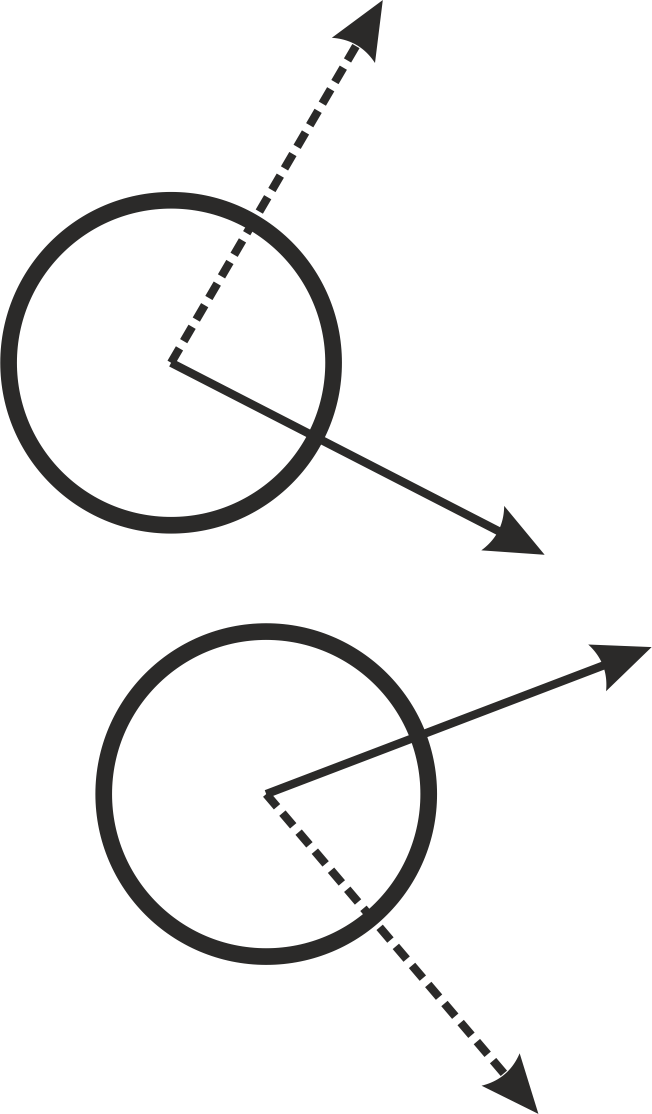
\includegraphics[height=200pt]{Images/NewtonInterractions}
                \caption{Парное взаимодействие в Ньютоновской жидкости}
        \end{subfigure}
        \begin{subfigure}{0.45\textwidth}
                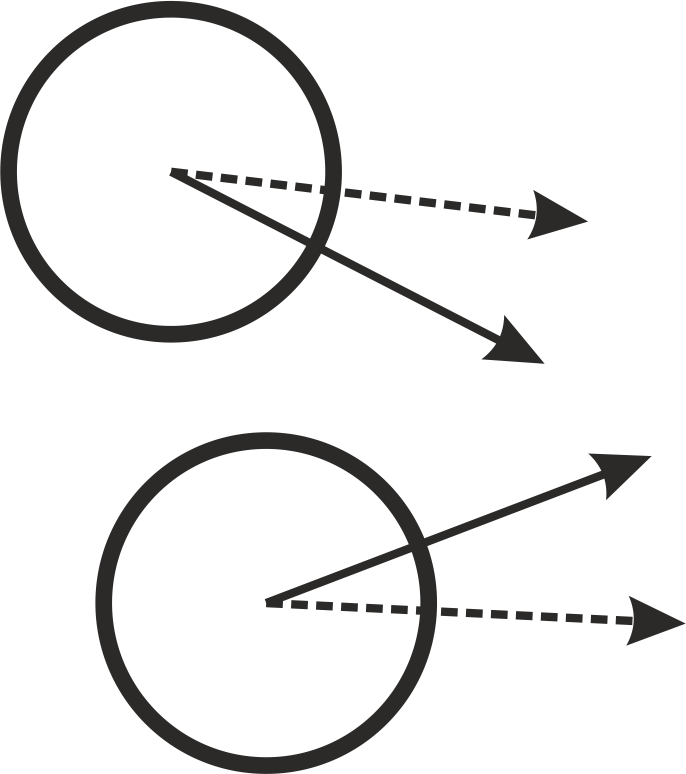
\includegraphics[height=200pt]{Images/VicsekInterrcations}
                \caption{Парное взаимодействие в Vicsek-подобной жидкости}
        \end{subfigure}
        \caption{Взаимодействие между частицами в разных моделях жидкости, непрерывная линия - направление скорости до взаимодействия, пунктирная - после.}
        \label{fig:PairParticleInterractions}
	\end{figure}

	Однако, как мы видим на рис.~\ref{fig:PairParticleInterractions}, для модели Vicsek'a, наоборот, выполняется увеличение упорядоченности при взаимодействии. Вопрос о роли шума в качестве стохастического хаоса остается открытым.
% section ClassicalModelsWIthViscosity (end)
